\documentclass[tikz]{standalone}

\usepackage{tikz}
\usetikzlibrary{positioning, arrows.meta, shapes, snakes, shadings}
\usepackage{amsmath,amssymb,amsthm,pgfplots}

\pgfmathdeclarefunction{gauss}{2}{%
  \pgfmathparse{1/(#2*sqrt(2*pi))*exp(-((x-#1)^2)/(2*#2^2))}
}

% polychrome colour, kelly
\definecolor{kwhite}{RGB}{242,243,244}
\definecolor{kred}{RGB}{175,35,55}
\definecolor{kyellow}{RGB}{236,195,66}
\definecolor{kblue}{RGB}{41,103,160}
\definecolor{kolivegreen}{RGB}{47,60,40}
\definecolor{kyellowgreen}{RGB}{150,180,55}
\definecolor{kpurplishpink}{RGB}{218,147,171}
\definecolor{korange}{RGB}{229,137,50}
\definecolor{kpurple}{RGB}{128,89,143}
\definecolor{kreddishbrown}{RGB}{126,51,31}
\definecolor{kgreen}{RGB}{59,133,90}
\definecolor{kbuff}{RGB}{192,178,134}
\definecolor{klightblue}{RGB}{169,201,237}
\definecolor{kyellowishpink}{RGB}{236,151,127}
\definecolor{kgrey}{RGB}{132,132,130}
\definecolor{kyellowishbrown}{RGB}{96,70,40}
\definecolor{kreddishorange}{RGB}{210,96,52}
\definecolor{kpurplishred}{RGB}{166,76,107}
\definecolor{kgreenishyellow}{RGB}{219,210,69}
\definecolor{korangeyellow}{RGB}{235,168,59}
\definecolor{kviolet}{RGB}{93,80,146}
\definecolor{kblack}{RGB}{34,34,34}

\begin{document}
    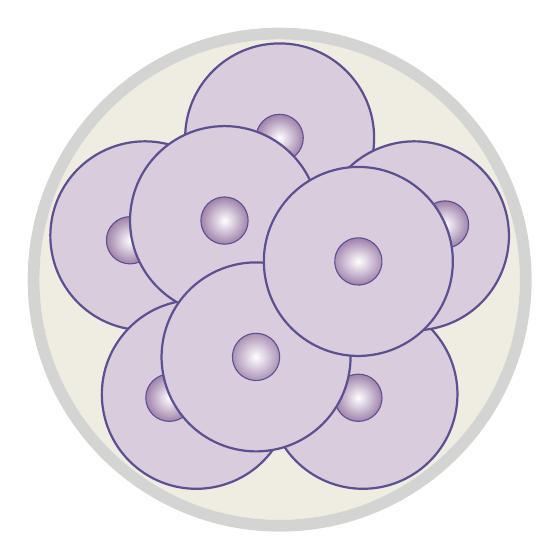
\begin{tikzpicture}
        % background
        \draw[draw=none, fill=kbuff!25] (3,3) circle[radius=3.05];
        
        % bottom blastomeres
        \foreach \x in {0,72,144,216,288}
        {
            \draw[draw=none, fill=kpurple!30, rotate around={\x:(3,3)}] (3,4.8) circle[radius=1.2];
            \draw[thick, draw=kviolet, rotate around={\x:(3,3)}] (3,4.8) circle[radius=1.2];
        }
        % manually draw nuclei of bottom blastomeres to be visible
        \draw[draw=kviolet, inner color=white, outer color=kpurple!75] (3,4.8) circle[radius=0.3];
        \draw[draw=kviolet, inner color=white, outer color=kpurple!75] (5.1,3.7) circle[radius=0.3];
        \draw[draw=kviolet, inner color=white, outer color=kpurple!75] (4,1.5) circle[radius=0.3];
        \draw[draw=kviolet, inner color=white, outer color=kpurple!75] (1.6,1.5) circle[radius=0.3];
        \draw[draw=kviolet, inner color=white, outer color=kpurple!75] (1.1,3.5) circle[radius=0.3];
        
        % top blastomeres
        \foreach \x in {0,120,240}
        {
            \draw[draw=none, fill=kpurple!30, rotate around={\x:(3,3)}] (2.3,3.75) circle[radius=1.2];
            \draw[thick, draw=kviolet, rotate around={\x:(3,3)}] (2.3,3.75) circle[radius=1.2];
            \draw[draw=kviolet, inner color=white, outer color=kpurple!75, rotate around={\x:(3,3)}] (2.3,3.75) circle[radius=0.3];
        }
%        \foreach \x in {0,120,240}
%        {
%            \draw[draw=none, kviolet, rotate around={\x:(3,3)}, fill=kpurple!50, opacity=.5] (3,4.5) arc[start angle=30, end angle=270, radius=1.5];
%            \draw[thick, kviolet, rotate around={\x:(3,3)}] (3,4.5) arc[start angle=30, end angle=270, radius=1.5];
%        }
%        %% nuclei
%        \foreach \x in {0,120,240}
%        {
%            \draw[draw=kviolet, inner color=white, outer color=kpurple!75, rotate around={-\x:(3,3)}] (1.5,4) circle[radius=0.4];
%        }
        
        % top blastomeres
%        \draw[draw=none, fill=kpurple!50, opacity=.5] (3,3) circle[radius=1.5];
%        \draw[thick, draw=kviolet] (3,3) circle[radius=1.5];
%        \draw[draw=kviolet, inner color=white, outer color=kpurple!75] (3.1,3.1) circle[radius=0.4];
%        
        % zona pellucida
        \draw[draw=none, fill=kgrey!35, even odd rule]
            (3,3) circle[radius=3.2] (3,3) circle[radius=3.05];
        
%        \draw[help lines, step=0.1] grid(6,6);
    \end{tikzpicture}   
\end{document}